\documentclass{beamer}

\usepackage[utf8]{inputenc}
\usepackage[english,russian]{babel}
\usepackage{cmap}
\hypersetup{unicode=true}
\usepackage{graphicx}
\graphicspath{{images/}{slides/images}}


\title{01. Lexical Statistics}
\subtitle{Computational Methods for Text Analysis}
\author{Пестова Алена}
\institute{НИУ ВШЭ Санкт-Петербург}

\newcommand{\tb}[1]{\colorbox{yellow}{#1}\space}
\newcommand{\Sp}[1]{\colorbox{green}{#1}\space}
\newcommand{\Sn}[1]{\colorbox{red}{#1}\space}

%\usetheme{lucid}
\begin{document}

    \begin{frame}
        \titlepage
    \end{frame}

    \begin{frame}{Assessment}
        \begin{equation}
            $$0.3 * \text{Final project} + 0.3 * \text{Homeworks} + 0.4 * \text{In-class participation}$$
        \end{equation}
    \end{frame}


    \begin{frame}{Topics}
        \begin{itemize}
            \item Text Preprocessing (preparing text for analysis)
            \item Contrastive Analysis (comparing texts
            \item Text Classification
            \item Word Embeddings (presenting word as a vector, how can we do that and why)
            \item (*) Language Models
        \end{itemize}
    \end{frame}

    \begin{frame}{Introduction}
        Computational Linguistics - is a field at the intersection of applied linguistics and computer science.
\\
        Tasks: automated processing of text. Very different tasks and methods -  from counting words to text generation.
\\
        In our course: methods of text analysis that can help to extract some information from texts for further research.

    \end{frame}

    

    \begin{frame}{How to count words?}

        If we want to estimate the word frequency distribution, we need to calculate the number of
        occurrences of each word (token) in the text.

        Tokenization - dividing text into tokens/words.

        Questions:

        \begin{itemize}
            \item What is a token? (What to count and what not to count?)
            \item Which tokens are considered as the same word?
        \end{itemize}
    \end{frame}

    \section{Tokenization}

\begin{frame}
\LARGE
  \frametitle{Tokenization}
\only<1>{
  \begin{block}{How many tokens?}
    Ой какие фотки<smile006><smile006><smile006> А разве роды в 38недель не считаются нормой?
  \end{block}
}
\only<2>{
  \begin{block}{11? (divide by spaces)}
    \tb{Ой} \tb{какие} \tb{фотки<smile006><smile006><smile006>} \tb{А} \tb{разве} \tb{роды} \tb{в} \tb{38недель} \tb{не} \tb{считаются} \tb{нормой?}
  \end{block}
}
\only<3>{
  \begin{block}{11? (take only words)}
    \tb{Ой} \tb{какие} \tb{фотки}<smile006><smile006><smile006> \tb{А} \tb{разве} \tb{роды} \tb{в} 38\tb{недель} \tb{не} \tb{считаются} \tb{нормой}?
  \end{block}
}
\only<4>{
  \begin{block}{13? (also considering punctuation)}
    \tb{Ой} \tb{какие} \tb{фотки} \tb{<smile006><smile006><smile006>} \tb{А}
    \tb{разве} \tb{роды} \tb{в} 38\tb{недель} \tb{не} \tb{считаются}
    \tb{нормой} \tb{?}
  \end{block}
}
\only<5>{
  \begin{block}{14? (delete the typo)}
    \tb{Ой} \tb{какие} \tb{фотки} \tb{<smile006><smile006><smile006>} \tb{А}
    \tb{разве} \tb{роды} \tb{в} \tb{38} \tb{недель} \tb{не} \tb{считаются}
    \tb{нормой} \tb{?}
  \end{block}
}
\only<6>{
  \begin{block}{16? (count smiles separately)}
    \tb{Ой} \tb{какие} \tb{фотки} \tb{<smile006>} \tb{<smile006>} \tb{<smile006>} \tb{А}
    \tb{разве} \tb{роды} \tb{в} \tb{38} \tb{недель} \tb{не} \tb{считаются}
    \tb{нормой} \tb{?}
  \end{block}
}
\end{frame}

\begin{frame}{Words Frequency}
    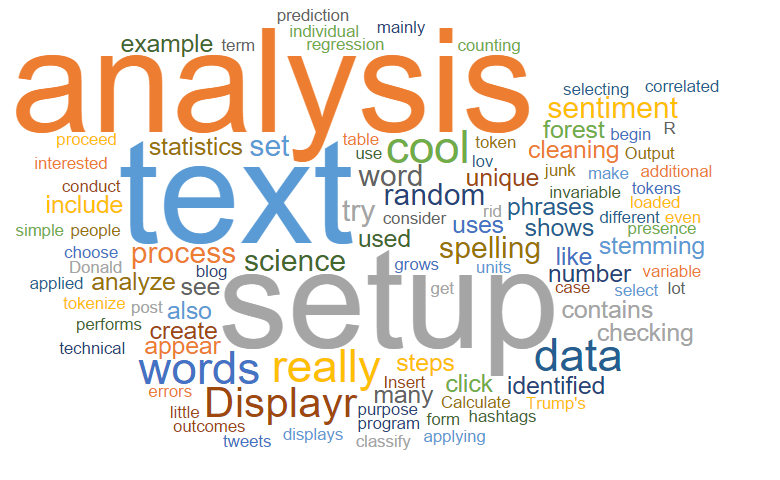
\includegraphics[width=\textwidth]{1setup-word-cloud.png}
\end{frame}


\begin{frame}{Words Frequency}
    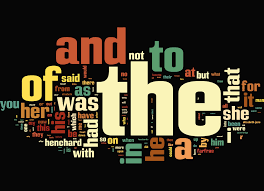
\includegraphics[width=\textwidth]{stopwords.png}
\end{frame}

    \begin{frame}{Zipf's Law}
        Zipf's Law (1949) predicts the frequency of the word by irs rank in the frequency list:

    \begin{equation}
      f(w) = \frac{C}{r(w)^a}
    \end{equation}
    \begin{itemize}
    \item[$f(w)$] — frequency of the word $w$
    \item[$r(w)$] — rank of the word $w$ in the frequency list
    \item[$C$] — constant
    \item[$a$] — constant (close to 1)
    \end{itemize}

    \end{frame}

    \begin{frame}{Zipf's Law}
         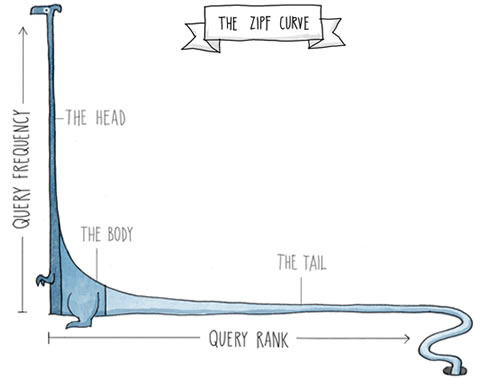
\includegraphics[width=\textwidth]{zipf-animal}

    \end{frame}

        \begin{frame}{Predictions of the Zipf's Law}

  If \structure{$a=1$}, \structure{$C=60000$} then by Zipf's Law:
  $$
       f(w) = \frac{60000}{r(w)}
  $$
 \begin{itemize}
  \item we will meet the most frequent word $f(w)=C/1=60000$ times
  \item the second - $C/2=30000$ times
  \item the third -  $C/3=20000$ times
  \item 100th - $C/100=600$ times
  \item 101st - $C/101=594,06$ times
  \item and we will have the long tail of 80000 words with the frequency between $1,5$ and $0,5$.
  \end{itemize}
\end{frame}

\begin{frame}
  \frametitle{Stop-words}
  The simplest way to decrease the number of lexical features is to delete the least informative words.

  \begin{itemize}
  \item Static List:

  \item Dynamic List:
    \begin{itemize}
    \item Too frequent (N most frequent; frequency greater than k)
    \item Too rare (frequency less than k)
    \item Too short (less than M letters)
    \item According to document frequency (present in more than k\%
      texts or less than k texts)
    \end{itemize}
  \end{itemize}
\end{frame}

\begin{frame}{Normalized Word Frequency}
 It is useful to represent counts on a normalized scale. A conventional unit for word frequencies in
corpus linguistics is IPM (Instances Per Million).

    $$\text{IPM} = \frac{\text{word frequency (count)}}{\text{number of words in the text / 1000000}}$$
\end{frame}























\end{document}